\chapter{Ugeopgave 10-11}
\label{cha:ugeopgave-10-11}

Denne ugeopgaves form�l var at g�re os bekendte med \emph{texture
  mapping}.

\section{Del 1}
\label{sec:del-1-3}

Vi har indsat \texttt{load\_ppm}-funktionen fra
forel�sningsslidesne\footnote{Desuden har vi rettet funktionen, s�
  den rent faktisk kan l�se \texttt{PPM}-filer ved at �ndre
  \emph{magic}-indl�sningen fra tre til to tegn.}. Samtidig har vi
gjort det muligt at angive en teksturfil n�r man laver en
\textsl{surface}.

\section{Del 2}
\label{sec:del-2-2}

Ud fra formlerne p� forel�sningsslidesne har vi beregnet de sf�riske
koordinater for et eventuelt sammenfaldspunkt mellem udsendte str�ler
og kuglen, men kun hvis sammenfaldspunktet endnu var det
n�rmeste. Disse har vi efterf�lgende skaleret til intervallet $[0;1]$
gemt i den udsendte str�le.

\section{Del 3}
\label{sec:del-3-2}

Teksturopslag er baseret p� de udregninger, der var givet p�
forel�sningsslidesne. Teksturkoordinaterne ($[0;1]\times[0;1]$) bliver omdannet
til billedkoordinater (fx $[[0;63]\times[0;63]$), hvorefter farverne
p� det koordinat bliver l�st ind og returneret.

Hvis der ikke er nogen teksturfil indl�st, returneres blot grundfarven
for objektet.

\section{Del 4}
\label{sec:del-4-2}

Ved tilf�jelse af teksturopslag i \texttt{shade}-funktionen fik vi et
billede, der kan ses p� figur \ref{fig:sphere}. Bem�rk, at
\emph{ambient} lys, \emph{lambertian}- og \emph{Phongshading} samt
reflektion og refraktion er fjernet fra raytraceren for bedre at kunne
se, om teksturerne blev indl�st korrekt.

\begin{figure}[htbp]
  \centering
  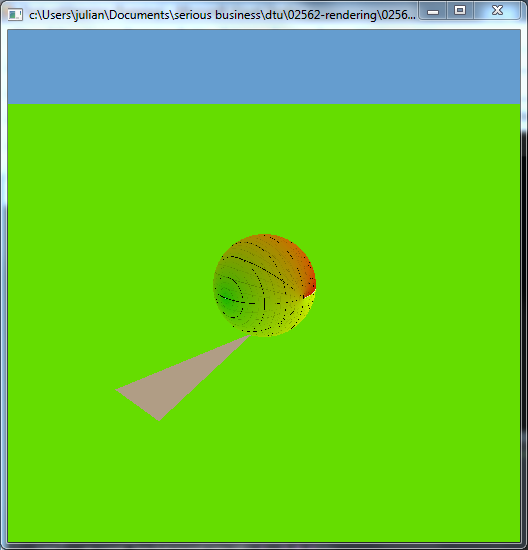
\includegraphics[width=8cm]{screenshots/exc10-11/sphere.png}
  \caption{Tekstur p� en kugle}
  \label{fig:sphere}
\end{figure}

\section{Del 5}
\label{sec:del-5-2}

For at \emph{mappe} trekantkoordinater til en firkantet tekstur laver
vi et par simplificeringer.

I det plan, der udsp�ndes af de trekanten g�r vi f�lgende:

\begin{itemize}
\item Den f�rst angivne knude i trekanten vil blive placeret i $(0,0)$.
\item Den n�ste angivne knude i trekanten vil blive placeret i
  $(X,0)$, hvor $X$ er l�ngden af vektoren fra den f�rste knude til
  denne knude.
\end{itemize}

Derefter beregner vi den tredje knudes placering i planet ud fra
vinklen mellem vektorerne $v_0 \rightarrow v_1$ og $v_0 \rightarrow
v_2$ samt l�ngden p� vektoren $v_0 \rightarrow v_2$.

Dern�st finder vi det mindste kvadrat, der kan indeholde hele
trekanten i planet. Hvert koordinat deles med kvadratsidel�ngden,
hvormed alle koordinater vil v�re i intervallet $[0;1]$.

Til sidst beregnes tekstur-koordinaterne, ved hj�lp af de barycentriske
koordinater, ud fra formlen givet p� forel�sningsslidesne.

Et billede af en trekant med en tekstur kan ses p� figur \ref{fig:triangle}.

\begin{figure}[htbp]
  \centering
  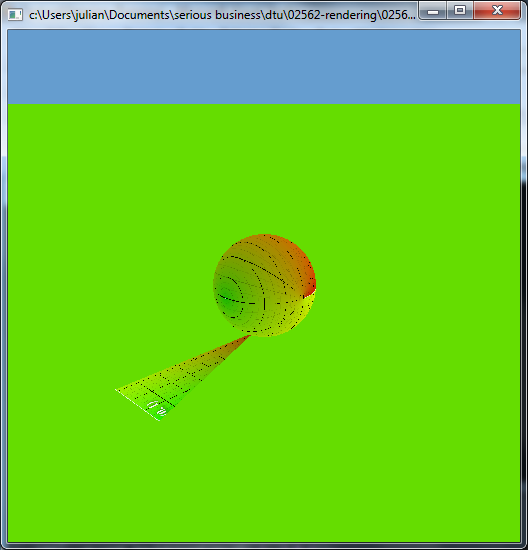
\includegraphics[width=8cm]{screenshots/exc10-11/triangle.png}
  \caption{Tekstur p� en trekant}
  \label{fig:triangle}
\end{figure}

%%% Local Variables: 
%%% mode: latex
%%% TeX-master: "report_main"
%%% End: 
